% This work is licensed under the Creative Commons
% Attribution-NonCommercial-ShareAlike 3.0 Unported License. To view a copy of
% this license, visit http://creativecommons.org/licenses/by-nc-sa/3.0/ or send
% a letter to Creative Commons, 444 Castro Street, Suite 900, Mountain View,
% California, 94041, USA.

\documentclass{mycourse}

\usepackage{xfrac}
\ExplSyntaxOn
\DeclareCollectionInstance{plainmath}{xfrac}{mathdefault}{math}
{
denominator-bot-sep = 0 pt,
numerator-bot-sep = 2 pt,
numerator-top-sep = \c_max_dim,
scaling = true,
scale-factor = 0.5,
h-scale = 0.7,
v-scale = 0.8,
slash-right-mkern = -3 mu,
slash-left-mkern = -3 mu,
}
\UseCollection{xfrac}{plainmath}
\ExplSyntaxOff

\usepackage{braket}

\usetikzlibrary{arrows,positioning}
\usepackage{tikz-cd}
\tikzset{
	commutative diagrams/sur/.style={two heads},
	commutative diagrams/inj/.style={hook},
	commutative diagrams/bij/.style={inj, sur},
	commutative diagrams/hom/.style={bij},
}

\newcommand{\B}{\mathbb{B}}
\newcommand{\D}{\mathbb{D}}
\renewcommand{\S}{\mathbb{S}}
\newcommand{\boundary}{\delta}
\newcommand{\dunion}{\sqcup}
\newcommand{\bigdunion}{\bigsqcup}
\newcommand{\oBdA}{o.B.d.A.}
\newcommand{\coursehref}[2]{\href{http://www.igt.uni-stuttgart.de/eiserm/lehre/2013/Topologie/Arbeitsblaetter/#1}{#2}}
\newcommand{\injto}{\hookrightarrow}
\newcommand{\surto}{\to}
\newcommand{\bijto}{\xrightarrow{\sim}}
\newcommand{\homeomorphic}{\cong}
\newcommand{\homto}{\xrightarrow{\homeomorphic}}
\newcommand{\eqq}{\equiv}
\newcommand{\homotopic}{\simeq}


\NewDocumentCommand \SepAxiom { m } {\ensuremath{\mathrm{T_{#1}}}}


%% no numbering
%\makeatletter
%\renewtheoremstyle{mythm}%
%	{\item[\rlap{\vbox{\hbox{\hskip\labelsep \theorem@headerfont
%			{\color{theoremtype}##1}\ \theorem@separator}\hbox{\strut}}}]}%
%	{\item[\rlap{\vbox{\hbox{\hskip\labelsep \theorem@headerfont
%			{\color{theoremtype}##1}\ \color{theoremtitle}(##3)\theorem@separator}\hbox{\strut}}}]}
%\makeatother

\renewtheorem{thm}{Theorem}[section]
\renewcommand{\thechapter}{\Alph{chapter}}
\renewcommand{\thesection}{\thechapter\relax\arabic{section}}


\begin{document}

\title{Topologie}

\maketitle

\tableofcontents

% Alphabetical
\chapter{Was ist und was soll die Topologie?}

\coursetimestamp{14}{10}{2013}

Dieser Frage wollen wir natürlich im Laufe der gesamten Vorlesung auf den Grund gehen.
Deshalb zunächst eine vorläufige Antwort: Topologie ist qualitative Geometrie.

\emph{Homöomorphie} gehört zu den Begriffen, mit denen die Topologie qualitative Aussagen über die Geometrie verschiedener Räume macht.

\begin{ex}
	% fixme: images
	Ränder von Dreiecken, Quadraten und Kreisen sind \emph{homöomorph}.
	Flächen von Dreiecken, Quadraten und Kreisen sind \emph{homöomorph}.
	Die Ränder sind jedoch nicht zu den Flächen homöomorph.
\end{ex}


\section{Zentrales Beispiel: Flächen}


% fixme: img: sphere, torus, …

\begin{df}
	Eine (berandete) \emph{Fläche} ist ein metrischer Raum, der lokal homöomorph ist zu
	\[
		\R^2_+ := \{ (x,y) \in \R^2 \suchthat x \ge 0 \}
	\]
\end{df}

\begin{ex}
	Zu $g \in \N, r \in \N_{\ge 1}$ betrachten wir
	\begin{align*}
		F_{g,r}^+ := % fixme: img
		F_{g,r}^- := % fixme: img
	\end{align*}
	% fixme: img: F_{0,1}^+, F_{0,2}^+, F_{0,1}^-

	% fixme: Definition für r=0
	Flächen ohne Rand: $F_g^+ := F_{g,0}^+$, $F_g^- := F_g^+ / \{\pm 1\}$.

	Diese Beispiele $F_{g,r}^{\pm}$ sind kompakte und zusammenhängende Flächen.

	Es stellen sich folgende Fragen
	\begin{enumerate}[1)]
		\item
			Ist unsere Liste vollständig?
		\item
			Ist unsere Liste redundanzfrei?
	\end{enumerate}
\end{ex}

\begin{ex}
	% fixme: img
	Sind diese Beispiele homöomorph zu $F_{g,r}^{\pm}$?
\end{ex}

\begin{st}[Klassifikation der kompakten Flächen]
	Jede kompakte, zusammenhängende Fläche $F$ ist homöomorph zu genau einem der Modelle $F_{g,r}^\pm$.
\end{st}

Wir werden in dieser Vorlesung wie folgt vorgehen:

\begin{enumerate}[1.]
	\item
		Analytische Topologie
	\item
		Geometrische Topologie
	\item
		Algebraische Topologie
\end{enumerate}

\chapter{Metrische Räume}

% paragraph B1
\section{Reelle Zahlen}

\begin{st}[Existenz und Eindeutigkeit der reellen Zahlen]
	Es existiert ein vollständiger, geordneter Körper $(\R,+,\cdot,<)$.

	Je zwei solcher Körper sind isomorph mittels eines eindeutig bestimmten Körperhomomorphismus.
\end{st}


\section{Skalarprodukt und Norm}

\begin{df}
	Sei $\K \in \{\R, \C\}$.
	Auf $V := \K^n$ definieren wir das \emph{Skalarprodukt}
	\[
		\<\argdot, \argdot\> : V \times V \to \K
	\]
	durch
	\[
		\<(x_1,\dotsc, x_n), (y_1,\dotsc, y_n)\> := \_{x_1}y_1 + \dotsb + \_{x_n}y_n.
	\]
	Es gelten
	\begin{enumerate}[({S}0)]
		\item
			$\<x,x\>  \in \R_{\ge 0}$
		\item
			$\<x,x\> > 0$ für $x \neq 0$
		\item
			$\<y,x\> = \_{\<x,y\>}$
		\item
			$\<x,\lambda y + \my z\> = \lambda \<x,y\> + \my\<x,z\>$.
	\end{enumerate}
	Jede Abbildung $V\times V \to \K$ mit (S0-3) ist ein Skalarprodukt.
\end{df}

\begin{ex}
	Sei $\Omega$ eine Menge, $\K^{\Omega} := \{f : \Omega \to \K\}$,
	\[
		\K^{(\Omega)} = \{ f: \Omega \to \K : f \text{ hat endlichen Träger} \}.
	\]
	Dann ist
	\[
		\<f,g\> := \sum_{x\in \Omega} \_{f(x)}g(x)
	\]
	ein Skalarprodukt
\end{ex}

\begin{ex}
	Auf $V = C([a,b], \C)$ ist
	\[
		\<f,g\> = \f 1{b-a} \int_{x-a}^b \_{f(x)} g(x) \dx
	\]
	ein Skalarprodukt.
\end{ex}



%fixme: \scr U vs U und \scr T vs \tau

\chapter{Topologische Räume}

\coursetimestamp{28}{10}{2013}

\begin{df}
	Eine \emph{Topologie} auf einer Menge $X$ ist ein System $\scr T \subset \scr P(X)$ von Teilmengen von $X$ mit folgenden Eigenschaften
	\begin{enumerate}[O1)]
		\item
			$\emptyset, X \in \scr T$,
		\item
			$O_1, \dotsc, O_n \in \scr T \implies O_1 \cap \dotsb \cap O_n \in \scr T$,
		\item
			$O_i \in \scr T$ für $i \in I \implies \bigcup_{i\in I} O_i \in \scr T$.
	\end{enumerate}
	Das Paar $(X, \scr T)$ nennen wir dann \emph{topologischer Raum}.
	Eine Teilmenge $Y \subset X$ nennen wir \emph{offen}, wenn $Y \in \scr T$, und \emph{abgeschlossen}, wenn $X \setminus Y \in \scr T$.
\end{df}

\begin{ex}[Kleinste Beispiele]
	\begin{itemize}
		\item
			$X = \emptyset, \scr T = \{\emptyset\}$,
		\item
			$X = \{a\}, \scr T = \{ \emptyset, X \}$,
		\item
			Für $x = \{a,b\}$ gibt es vier Topologien
			\begin{enumerate}[1.]
				\item
					$\{\emptyset, X\}$
				\item
					$\{\emptyset, \{a\}, X\}$
				\item
					$\{\emptyset, \{b\}, X \}$
				\item
					$\{\emptyset, \{a\}, \{b\}, X\}$
			\end{enumerate}
	\end{itemize}
	\begin{table}
		\centering
		\caption{Anzahl der Topologien auf einer Menge $X$ mit $n$ Elementen, asymptotisches Verhalten: $\log t_n \sim \f {n^2}4$}
		\begin{tabular}{c|c}
			$n=|x|$ & $t_n = $ Anzahl der Topologie auf $X$ \\ \hline
			0 & 1 \\
			1 & 1 \\
			2 & 4 \\
			3 & 29 \\
			4 & 355 \\
			5 & 6942
		\end{tabular}
	\end{table}
\end{ex}

\begin{ex}[diskrete Topologie]
	$\scr T = \scr P(X)$ auf $X$.
\end{ex}

\begin{ex}[indiskrete Topologie]
	$\scr T = \{\emptyset, X\}$ auf $X$.
\end{ex}

\begin{ex}[metrische Topologie] \label{ex:metric_topology}
	Die metrische Topologie zu einer (Halb-)Metrik $d: X \times X \to [0,\infty]$ ist gegeben durch
	\begin{align*}
		\scr T_d
		&= \{ O \subset X : \forall a \in O \exists \eps > 0 : B(a,\eps) \subset O \} \\
		&= \{ O \subset X : \forall a \in O \exists \eps > 0 : d(a,x) < \eps \implies x \in O \}.
	\end{align*}
\end{ex}

\begin{nt}
	% fixme: reference
	Die offenen Mengen einer metrischen Topologie entsprechen den offenen Mengen aus dem letzten Kapitel.
\end{nt}

\begin{df}[metrisierbare Topologie]
	Eine Topologie $\scr T$ heißt \emph{metrisierbar}, wenn es eine Metrik $d$ gibt mit $\scr T = \scr T_d$.
\end{df}

\begin{ex}
	Die diskrete Topologie ist metrisierbar (dank der diskreten Metrik).

	Die indiskrete Topologie hingegen nicht (für $|x| \ge 2$).
	(Jede metrische Topologie trennt je zwei Punkte $a \neq b$, die indiskrete Topologie tut das nicht)
\end{ex}

\begin{df}
	Sind $\scr T_1 \subset \scr T_2 \subset \scr P(X)$ Topologien auf $X$, so nennen wir $\scr T_1$ \emph{gröber} als $\scr T_2$, bzw. $\scr T_2$ \emph{feiner} als $\scr T_1$.
\end{df}

\begin{ex}
	Sei $(X,<)$ eine linear geordnete Menge, z.B. $(\R,<)$.
	Wir nennen $O \subset X$ offen, wenn zu jedem $x \in O$ ein offenes Intervall $I \subset X$ existiert mit $x \in I \subset O$.
	Das System $\scr T_<$ dieser offener Mengen heißt \emph{Ordnungstopologie} von $(X,<)$.
\end{ex}

\begin{ex}[Koendliche Topologie auf $X$]
	Setze
	\[
		\scr T
		:= \{ O \subset X : X \setminus O \text{ ist endlich} \} \cup \{\emptyset\}.
	\]
\end{ex}

\begin{ex}[Koabzählbare Topologie auf $X$]
	Setze
	\[
		\scr T
		:= \{ O \subset X : X \setminus O \text{ ist abzählbar} \} \cup \{ \emptyset \}.
	\]
\end{ex}

\begin{nt}
	Es gilt stets
	\[
		\scr T_{\text{indiskret}}
		\subset \scr T_{\text{koendlich}}
		\subset \scr T_{\text{koabzählbar}}
		\subset \scr T_{\text{diskret}}
	\]
	(nach links hin gröber, nach rechts hin gröber).
\end{nt}

\begin{df}
	Eine Abbildung $f: (X,\scr T_X) \to (Y, \scr T_Y)$ heißt \emph{stetig}, wenn aus $V \in \scr T_Y$ stets $f^{-1}(V) \in \scr T_X$ folgt.

	Hingegen heißt $f$ \emph{offen}, wenn aus $U \in \scr T_X$, stets $f(X) \in T_Y$ folgt und \emph{abgeschlossen}, wenn aus $X \setminus A \in \scr T_X$ stets $Y \setminus f(A) \in \scr T_Y$ folgt.
	\begin{nt}
		Diese Eigenschaften sind voneinander unabhängig:
		\begin{itemize}
			\item
				$\Id_\R: \R \to \R$ hat alle Eigenschaften,
			\item
				$f: \R \to \R, f(x) = x^2$ ist stetig, abgeschlossen, aber nicht offen,
			\item
				$f: \R \to \R, f(x) = \arctan(x)$ ist stetig, offen, aber nicht abgeschlossen,
			\item
				$f: \R \to \R, f(x) = \f 1{1+x^2}$ ist stetig, aber weder offen, noch abgeschlossen,
			\item
				\dots
		\end{itemize}
	\end{nt}
\end{df}

\begin{df}
	Eine Homöomorphismus $f: (X,\scr T_X) \to (Y, \scr T_Y)$ ist eine bijektive Abbildung $f: X \to Y$, sodass $f$ und $f^{-1}$ stetig sind.
\end{df}

\begin{nt}
	Aus der Stetigkeit von $f$ folgt im Allgemeinen nicht die Stetigkeit von $f^{-1}$.
	Betrachte dazu $f: [1,2[ \cup [3,4] \to [1,3[$ mit
	\[
		f(x) = \begin{cases}
			x & x \in [1,2[ \\
			x - 1 & x \in [3,4[
		\end{cases}.
	\]
	$f$ ist bijektiv, stetig, aber kein Homöomorphismus.
	Oder: $f : [0,1[ \to \S^1 \subset \C$ definiert durch
	\[
		f(t)
		= e^{2\pi i t}
		= (\cos (2\pi t), \sin (2\pi t))
	\]
	ist bijektiv, stetig, aber kein Homöomorphismus (es gibt sogar kein Homöomorphismus zwischen $[0,1[$ und $\S^1$).
\end{nt}


\section{Umgebungen}


Sei im folgenden $(X, \scr T)$ ein topologischer Raum, $x \in X$.

\begin{df}
	Eine Menge $\scr O$ heißt \emph{offene Umgebung} von $x$ in $(X,\scr T)$, wenn $x \in O \in \scr T$ gilt.
	\[
		U_x^O = U_x^O(\scr T)
		:= \{ O \in \scr T : x \in O \}
	\]

	Eine Menge $U$ heißt \emph{Umgebung} von $x$ in $(X, \scr T)$, wenn sie eine offene Umgebung von $x$ enthält
	\[
		U_x = U_x(\scr T)
		:= \{ U \subset X : \exists O \in \scr T : x \in O \subset U \}
	\]
\end{df}

\begin{df}
	Eine Familie $\scr B_x \subset U_x$ heißt \emph{Umgebungsbasis} von $x$ in $(X, \scr T)$, wenn jede Umgebung $U$ von $x$ eine Umgebung $V \in \scr B_A$ enthält.

	Dann ist
	\[
		U_x = \{ U \subset X : \exists V \in \scr B_x : V \subset U \}.
	\]
\end{df}

\begin{ex}
	\begin{itemize}
		\item
			$U_x$ ist eine Umgebungsbasis, ebenso $U_x^O$.
		\item
			In jedem metrischen Raum $(X,d)$ bilden die Bälle $B(a,\eps)$ mit $\eps > 0$ eine Umgebungsbasis von $a$, ebenso $B(a, \f 1k)$ mit $k= 1, 2, \dotsc$,
			diese ist sogar abzählbar.
	\end{itemize}
\end{ex}

\begin{df}
	Ein topologischer Raum $(X, \scr T)$ erfüllt das \emph{erste Abzählbarkeitsaxiom} (1AA), wenn jeder Punkt $a \in X$ eine abzählbare Umgebungsbasis besitzt.
	\begin{nt*}
		Hat $a$ eine abzählbare Umgebungsbasis $(V_n)_{n\in\N}$, so auch eine offene Umgebungsbasis, etwa $(\mathring V_n)_{n\in\N}$.

		Durch Übergang zu $U_n := \mathring V_0 \cap \dotsb \cap \mathring V_n$ erhalten wir eine offene Basis $U_0 \supset U_1 \supset U_2 \supset \dotsb$.
	\end{nt*}
\end{df}

\begin{ex}
	\begin{itemize}
		\item
			Jeder metrische Raum erfüllt das 1AA.
		\item
			Auf einer überabzählbaren Menge $X$, etwa $X = \R$, erfüllen die koendliche und die koabzählbare Topologie nicht das 1AA.
			Diese können also nicht metrisiert werden.
	\end{itemize}
\end{ex}

\begin{df}
	Eine Folge $(x_n)_{n\in \N}$ in $X$ \emph{konvergiert} gegen $a \in X$ bezüglich $\scr T$, wenn jede Umgebung $U$ von $a$ in $(X, \scr T)$ fast alle Folgenglieder enthält:
	\[
		(x_n)_{n\in \N} \stack{\scr T}\to a
		\iff
		\forall U \in \scr U_a(\scr T) \exists m \in \N \forall n \ge m : x_n \in U
	\]
\end{df}

\begin{prop}
	Eine Folge $(x_n)$ in $X$ konvergiert gegen $a \in X$ genau dann, wenn
	\[
		\forall V uin \scr B_x \exists m \in \N \forall n \ge m : x_n \in V.
	\]
\end{prop}

Grenzwerte sind im Allgemeinen nicht eindeutig, betrachte dazu folgendes Beispiel

\begin{ex}
	Ist $(X, \{\emptyset, X\})$ ein indiskreter Raum, so konvergiert jede Folge gegen jeden beliebigen Punkt $a \in X$.
\end{ex}

\begin{df}
	Ein topologischer Raum $(X, \scr T)$ heißt \emph{hausdorffsch}, wenn zu je zwei Punkten $a \neq b$ in $X$ disjunkte Umgebungen existieren, d.h. $U \in \scr U_a, V \in \scr U_b$, so dass $U \cap V = \emptyset$.
\end{df}

\begin{ex}
	Jeder metrische Raum ist hausdorffsch.
\end{ex}

\begin{st}
	Ist $(X,\scr T)$ hausdorffsch, dann hat jede Folge in $X$ höchstens einen Grenzwert in $X$.

	Die Umkehrung gilt, wenn $(X, \scr T)$ das erste Abzählbarkeitsaxiom erfüllt.
	\begin{proof}
		Aus $x_n \to a$ und $y_n \to b$ folgt $a = b$ (mit $U \in \scr U_a, V \in \scr U_b, U \cap V = \emptyset$ folgt der Widerspruch).
	\end{proof}
\end{st}

% D
\chapter{Kompaktheit}



\section{Grundlagen}


\begin{df}[Kompakter topologischer Raum] \label{df:compact_space}
	Ein topologischer Raum $(X, \scr T)$ heißt \emph{kompakt}, wenn zu $X = \bigcup_{i\in I} U_i$ mit $U_i \in \scr T$ endlich viele Indizes $i_1, \dotsc, i_n \in I$ existieren mit $X = \bigcup_{k=1}^n U_{i_k}$.
\end{df}

\begin{ex}
	\begin{itemize}
		\item
			Jeder Raum mit indiskreter Topologie ist kompakt.
		\item
			$\R^n = \bigcup_{n\in\N} B(0,n)$ enthält keine endliche Teilüberdeckung, $\R^n$ ist also mit euklidischer Topologie nicht kompakt.
		\item
			Für einen diskreten Raum $(X, \scr T)$ gilt:
			\[
				(X, \scr T) \text{ kompakt }
				\iff
				\text{ $X$ endlich}.
			\]
	\end{itemize}
\end{ex}

\begin{df}[Kompakte Teilmenge/Kompakter Teilraum] \label{df:compact_subspace}
	\begin{enumerate}[(1)]
		\item
			$A \subset X$ heißt \emph{kompakt in $(X, \scr T_X)$}, wenn jede offene Überdeckung von $A$, $\bigcup_{i\in I} U_i \supset A$, mit $U_i \in \scr T_X$ eine endliche Teilüberdeckung enthält.
		\item
			$A \subset X$ heißt \emph{relativ kompakt in $(X, \scr T_X)$}, wenn $\_A$ in $(X, \scr T_X)$ kompakt ist.
	\end{enumerate}
\end{df}

\begin{nt}
	Sei $(A, \scr T_A)$ ein Teilraum von $(X, \scr T)$.
	$K \subset A$ ist kompakt in $(X, \scr T)$ genau dann, wenn $K$ kompakt in $(A, \scr T_A)$ ist.

	Insbesondere ist der Teilraum $(A, \scr T_A)$ genau dann kompakt (gemäß \ref{df:compact_space}), wenn $A \subset X$ in $(X, \scr T_X)$ kompakt ist (gemäß \ref{df:compact_subspace}).
	\begin{proof}
		\begin{segnb}[„$\implies$“]
			Sei $\bigcup_{i\in I} U_i \supset K, U_i \in \scr T_A$ eine offene Überdeckung von $K$ in $(A, \scr T_A)$.
			Nach Definition des Teilraums existieren $V_i \in \scr T : U_i = V_i \cap A$ für alle $i \in I$.
			\[
				\bigcup_{i\in I} V_i
				\supset A \cap \bigcup_{i\in I} V_i
				= \bigcup_{i\in I} \underbrace{(V_i \cap A)}_{= U_i}
				\supset K
			\]
			ist eine offene Überdeckung von $K$ in $(X, \scr T_X)$ mit endlicher Teilüberdeckung $\bigcup_{k=1}^n V_{i_k} \supset K$.
			Also ist
			\[
				\bigcup_{k=1}^n \underbrace{U_{i_k}}_{= V_{i_k} \cap A}
				= A \cap \bigcup_{k=1}^n V_{i_k}
				\supset A \cap K
				= K
			\]
			eine endliche Teilüberdeckung von $\bigcup_{i\in I} U_i \supset K$.
		\end{segnb}
		\begin{segnb}[„$\impliedby$“]
			Sei $\bigcup_{i\in I} U_i \supset K, U_i \in \scr T$ eine offene Überdeckung von $K$ in $(X, \scr T)$ und $V_i := A \cap U_i \in \scr T_A$ für $i \in I$.
			\[
				\bigcup_{i\in I} \underbrace{V_i}_{=A \cap U_i}
				= A \cap \bigcup_{i\in I} U_i
				\supset A \cap K
				= K
			\]
			ist eine offene Überdeckung von $K$ in $(A, \scr T_A)$ mit endlicher Teilüberdeckung $\bigcup_{k=1}^n V_{i_k} \supset K$.
			Also ist
			\[
				\bigcup_{k=1}^n U_{i_k}
				\supset A \cap \bigcup_{k=1}^n U_{i_k}
				= \bigcup_{k=1}^n \overbrace{V_{i_k}}^{=A \cap U_{i_k}}
				\supset K
			\]
			eine endliche Teilüberdeckung von $\bigcup_{i\in I} U_i \supset K$.
		\end{segnb}
	\end{proof}
\end{nt}

\begin{ex}
	\begin{itemize}
		\item
			Jede endliche Menge $A \subset X$ ist kompakt.
		\item
			$\Z \subset \R$ ist nicht kompakt, ebensowenig $\Q \subset \R$.
		\item
			$]0,1] \subset \R$ ist nicht kompakt, aber relativ kompakt in $\R$, denn $\_{]0,1]} = [0,1]$ (Abschluss in $\R$).
	\end{itemize}
\end{ex}

\begin{st}[Kompakte Ordnungstopologie, Charakterisierung]
	Sei $(X, <)$ ein geordnete Menge.
	Genau dann ist jedes Intervall $[a,b]$ in $X$ kompakt bezüglich der Ordnungstopologie, wenn $(X, <)$ vollständig geordnet ist (d.h. $(X,<)$ erfüllt das Supremums-Axiom).
\end{st}

\begin{ex}
	\begin{itemize}
		\item
			$(\R, <)$ ist vollständig geordnet und jedes Intervall $[a,b] \subset \R$ ist kompakt.
		\item
			$(\Q, <)$ ist nicht vollständig geordnet und jedes Intervall $[a,b]_\Q$ mit $a<b$ ist nicht kompakt.

			Sei $\xi \in [0,1] \setminus \Q$, z.B. $\xi = \f{\sqrt 2}2$.
			Dann bilden
			\begin{align*}
				S_n &= [0, \xi - \f 1n[_{\Q},&
				T_n &= ]\xi + \f 1n, 1]_{\Q}
			\end{align*}
			eine offene Überdeckung $[0,1]_{\Q} = \bigcup_{n\in\N} S_n \cup \bigcup_{n\in\N} T_n$ ohne endliche Teilüberdeckung.
	\end{itemize}
\end{ex}

\begin{lem} \label{lem:hausdorff_compact_subspace_neighbourhood}
	Sei $(X, \scr T)$ hausdorffsch, $A \subset X$ kompakt und $b \in X \setminus A$.
	Dann existieren offene Umgebungen $U$ von $A$ in $X$ und $V$ von $b$ in $X$ mit $U\cap V = \emptyset$.
	\begin{proof}
		Zu $a \in A$ existieren $a \in U_a \in \scr T$ und $b \in V_a \in \scr T$ mit $U_a \cap V_a = \emptyset$.
		Da $A$ kompakt, gilt $A \subset U_{a_1} \cup \dotsb \cup U_{a_n} =: U$ und $V := V_{a_1} \cap \dotsb \cap V_{a_1} \ni b$.
	\end{proof}
\end{lem}

\begin{st}
	Sind $A, B$ kompakt mit $A \cap B = \emptyset$ in einem Hausdorff-Raum $(X, \scr T)$, dann existieren $A \subset U \in \scr T$ und $B \subset V \in \scr T$ mit $U \cap V = \emptyset$.
	\begin{proof}
		Analog zu oben.
	\end{proof}
\end{st}

\coursetimestamp{18}{11}{2013}

\begin{st}
	In jedem kompakten Raum $(X, \scr T)$ ist jede abgeschlossene Teilmenge $A \subset X$ kompakt.
	\begin{proof}
		Sei $A \subset \bigcup_{i\in I} U_i$ mit $U_i \in \scr T$, dann ist
		\[
			X
			= (X \setminus A) \cup \bigcup_{i\in I} U_i
			= (X \setminus A) \cup U_{i_1} \cup \dotsb \cup U_{i_n},
		\]
		also $A \subset U_{i_1} \cup \dotsb \cup U_{i_n}$.
	\end{proof}
\end{st}

\begin{st}
	In einem Hausdorff-Raum $(X, \scr T)$ ist jede kompakte Teilmenge $A \subset X$ abgeschlossen.
	\begin{proof}
		Nach \ref{lem:hausdorff_compact_subspace_neighbourhood} findet sich zu jedem $b \in X \setminus A$ eine offene Umgebung in $X \setminus A$.
	\end{proof}
\end{st}

\subsection{Kompaktheit unter Abbildungen}

\begin{st}
	Ist $X$ kompakt, $f: X \to Y$ stetig, dann ist $f(X) \subset Y$ kompakt.
	\begin{proof}
		Sei $f(X) \subset \bigcup_{i\in I} V_i$ mit $V_i \in \scr T_y$.
		Da $f$ stetig ist
		\[
			U_i = f^{-1}(V_i) \in \scr T_X
		\]
		und $X = \bigcup_{i\in I} U_i = \bigcup_{k=1}^n U_{i_k}$
		Aus $f(U_i) \subset V_i$ folgt
		\[
			f(X)
			\subset f(U_{i_1}) \cup \dotsb \cup f(U_{i_n})
			\subset V_{i_1} \cup \dotsb \cup V_{i_n}.
		\]
	\end{proof}
\end{st}

\begin{st}
	Ist $X$ kompakt, $f: X \to \R$ stetig, so existieren $a, b \in X$ mit
	\[
		f(a) \le f(x) \le f(b)
	\]
	für alle $x \in X$.
	\begin{proof}
		Leicht nachvollziehbar.
	\end{proof}
\end{st}

\begin{st}
	Sei $X$ kompakt, $Y$ hausdorffsch.
	Dann ist jede stetige Abbildung $f: X \to Y$ abgeschlossen und induziert in der kanonischen Faktorisierung ein Homöomorphismus $\_f$.
	\[
		\begin{tikzcd}
			X \arrow{r}{f} \arrow[sur]{d}{q} & Y \\
			X / R_f \arrow{r}{\_f} & f(X) \arrow[inj]{u}{\jota}
		\end{tikzcd}
	\]
	\begin{proof}
		Sei $A \subset X$ abgeschlossen.
		Da $X$ kompakt, ist auch $A$ kompakt und damit wegen Stetigkeit von $f$ auch $f(A)$.
		Da $Y$ hausdorffsch, ist also auch $f(A)$ abgeschlossen.
	\end{proof}
\end{st}

\begin{ex}
	Wir wissen $\R / \Z \homto \scr S^1$.
	Die Abbildung $p: \R \to \S^1$ mit $p(t) = e^{2\pi i t}$ ist stetig, surjektiv und $p(x) = p(x') \iff x-x' \in \Z$.
	In der kanonischen Faktorisierung erhalten wir
	\[
		\begin{tikzcd}
			\R \arrow{d}{q} \arrow{r}{p} & \S^1 \\
			\R / \Z \arrow{r}{\_p} & \S^1 \arrow{u}
		\end{tikzcd}.
	\]
	Da $\R / \Z = q([0,1])$ kompakt ist und $\S^1 \subset \R^2$ hausdorffsch, ist $\_p$ ein Homöomorphismus.
\end{ex}

\begin{ex}
	$\D^n / \S^{n-1} \homeomorphic \S^n$
\end{ex}

\subsection{Summen}

\begin{st}
	Sei $(X_\lambda)_{\lambda\in\Lambda}$ eine Familie topologischer Räume mit $X_\lambda \neq \emptyset$.
	Die Summe $X = \bigdunion_{\lambda \in \Lambda} X_\lambda$ ist genau dann kompakt, wenn alle $X_\lambda$ kompakt sind und $\Lambda$ endlich ist.
	\begin{proof}
		\begin{segnb}[„$\impliedby$“]
			klar
		\end{segnb}
		\begin{segnb}[„$\implies$“]
			Angenommen $X_\lambda$ offen, dann ist $X = \bigcup_{\lambda\in\Lambda} X_\lambda$ offene Überdeckung ohne echte Teilüberdeckung.
			Also ist $X_\lambda$ abgeschlossen in $X$, also kompakt.
			% fixme: prüfen
		\end{segnb}
	\end{proof}
\end{st}

\subsection{Charakterisierung durch Filter}

\begin{st}
	Ein topologischer Raum $(X, \scr T)$ ist genau dann kompakt, wenn jeder Ultrafilter $\scr F$ auf $X$ konvergiert, also ein $x \in X$ existiert mit $\scr F \supset \scr U_x$.
	\begin{proof}
		\begin{segnb}[„$\implies$“]
			Sei $X$ kompakt und $\scr F$ ein Ultrafilter.
			Angenommen $\scr F$ konvergiert nicht, d.h. jeder Punkt $x \in X$ hat eine offene Umgebung $x \in U_x \in \scr T$ mit $U_x \not\in \scr F$.
			Da $X$ kompakt, existiert eine Überdeckung $X = U_{x_1} \cup \dotsb \cup U_{x_n}$ mit $U_{x_1}, \dotsc, U_{x_n} \not\in \scr F$.
			Da $\scr F$ ein Ultrafilter ist, gilt $X \setminus U_{x_1}, \dotsc, X \setminus U_{x_n} \in \scr F$.
			Nach (F2) ist
			\[
				(X \setminus U_{x_1}) \cap \dotsc \cap (X \setminus U_{x_n})
				= X \setminus (U_{x_1} \cup \dotsc \cup U_{x_n})
				= \emptyset \in \scr F,
			\]
			ein Widerspruch zu (F1).
		\end{segnb}
		\begin{segnb}[„$\impliedby$“]
			Angenommen $X$ ist nicht kompakt, d.h. es existiert $X = \bigcup_{i\in I} U_i$, $U_i \in \scr T$ ohne endliche Teilüberdeckung.
			Dann ist
			\[
				\scr E
				= \Set{ X \setminus \bigcup_{i\in J} U_i | J \subset I \text{ endlich} }
			\]
			eine Filterbasis.
			Diese erzeugt einen Filter und dieser liegt in einem Ultrafilter $\scr F$ auf $X$.
			Nach Voraussetzung konvergiert $\scr F$ gegen ein $x \in X$, d.h. $\scr F \supset \scr U_x$.
			Wegen $X = \bigcup_{i\in I} U_i$ existiert $j \in I$ mit $x \in U_j \in \scr T$, also $U_j \in \scr U_x \subset \scr F$.
			Andererseits gilt $X \setminus U_j \in \scr E \subset \scr F$.
			Nach (F2) ist also $U_j \cap (U \setminus U_j) = \emptyset \in \scr F$, ein Widerspruch zu (F1).
		\end{segnb}
	\end{proof}
\end{st}

\subsection{Produkte}

\begin{st}[Tychonoff, 1930]
	Seien $(X_i, \scr T_i)_{i\in I}$ nicht-leere topologische Räume.
	Der Produktraum $(X, \scr T) = \prod_{i\in I} (X_i, \scr T_i)$ ist kompakt genau dann, wenn jeder Raum $(X_i, \scr T_i)$ kompakt ist.
	\begin{proof}
		\begin{segnb}[„$\implies$“]
			$p_i: X \to X_i$ ist stetig und surjektiv, also ist $X_i$ kompakt.
		\end{segnb}
		\begin{segnb}[„$\impliedby$“]
			Sei $\scr F$ ein Ultrafilter auf $X$.
			Dann ist $p_i(\scr F)$ ein Ultrafilter auf $X_i$ (Übungsaufgabe). % fixme: ref
			Da $X_i$ kompakt, existiert $x_i \in X_i$ mit $p_i(\scr F) \to x_i$.
			Dann konvergiert $\scr F$ auf $X$ gegen $x = (x_i)_{i\in I}$.
		\end{segnb}
	\end{proof}
\end{st}

\begin{ex}
	\begin{itemize}
		\item
			$\{0,1\}^\N$ ist kompakt.
		\item
			$[a_1,b_1] \times \dotsb \times [a_n,b_n] \subset \R^n$ ist kompakt.
		\item
			$\prod_{k\in\N} [a_k,b_k] \subset \R^\N$ ist kompakt.
		\item
			$\prod_{x\in\R} [a_x,b_x] \subset \R^\R$ ist kompakt.
	\end{itemize}
\end{ex}

\begin{ex}[Hilbert-Würfel]
	Der Hilbert-Würfel $[0,1]^\N$ ist kompakt und metrisierbar.
	Ebenso in $\ell^2(\N)$ ist der Hilbert-Quader
	\[
		H = \Set{ f: \N \to \R | \le f(k) \le \f 1{k+1} }
		= [0,1] \times [0,\f 12] \times [0, \f 13] \times \dotsb
	\]
	Es gilt $H \homeomorphic [0,1]^\N$.
\end{ex}

\begin{st}[verwandte Kompaktheitsbegriffe]
	Für topologische Räume gilt
	\begin{itemize}
		\item
			Kompaktheit impliziert abzählbare Kompaktheit
		\item
			abzählbare Kompaktheit impliziert Kompaktheit unter Voraussetzung des zweiten Abzählbarkeitsaxioms
		\item
			Folgenkompaktheit impliziert abzählbare Kompaktheit
		\item
			abzählbare Kompaktheit impliziert Folgenkompaktheit unter Voraussetzung des ersten Abzählbarkeitsaxioms.
		\item
			Abzählbare Kompaktheit impliziert Pseudokompaktheit
	\end{itemize}
	\begin{proof}
		Wie im metrischen Fall.
		% fixme: ref
	\end{proof}
\end{st}


\section{Lokale Kompaktheit}


\begin{df}
	Ein Raum $(X, \scr T)$ heißt \emph{lokal-kompakt}, wenn jede Umgebung eines Punktes eine kompakte Umgebung enthält, d.h.
	\[
		\forall x \in X \forall U \in \scr U_x \exists K \in \scr U_x : \text{$K \subset U$ und $K$ kompakt}.
	\]
\end{df}

\begin{ex}
	\begin{itemize}
		\item
			$\R^n$ ist lokal-kompakt.
		\item
			Kein Punkt $x\in \Q$ besitzt eine kompakte Umgebung, insbesondere ist also $\Q$ nicht lokal-kompakt.
	\end{itemize}
\end{ex}

\begin{st} \label{st:hausdorff_compact_neighbourhoods_locally_compact_space}
	Sei $(X, \scr T)$ ein Hausdorff-Raum und zu jedem Punkt $x \in X$ existiere eine kompakte Umgebung.
	Dann ist $(X, \scr T)$ lokal-kompakt.
	\begin{proof}
		Sei $x \in X$ und $K \in \scr U_x$ kompakt.
		Zu jeder offenen Umgebung $U \in \scr U_x$ müssen wir eine kompakte Umgebung $K_U \in \scr U_x$ mit $K_U \subset U$ finden.

		Setze
		\[
			A := K \setminus U
		\]
		($A$ kompakt) und seien $V, W$ offene Umgebungen von $x$, bzw. $A$ mit $V \cap W = \emptyset$ (Hausdorff-Eigenschaft).
		Setze
		\[
			K_U := K \setminus W
		\]
		$K_U$ ist abgeschlossen und kompakt und zudem eine Umgebung von $x$, denn $x \in K \cap V \subset K \setminus W = K_U$.
		Weiterhin gilt $K_U \subset U$.
	\end{proof}
\end{st}

\begin{kor}
	Jeder kompakte Hausdorff-Raum ist lokal-kompakt.
	\begin{proof}
		Der Raum ist kompakte Umgebung eines jeden seiner Punkte, also folgt die Aussage direkt mit \ref{st:hausdorff_compact_neighbourhoods_locally_compact_space}.
	\end{proof}
\end{kor}

\begin{lem}
	Ist $(X, \scr T)$ lokal-kompakt, so auch jeder offene und jeder abgeschlossene Teilraum.
	\begin{proof}
		Für einen Teilraum $(O, \scr T_O)$ mit beliebigem $x \in O \in \scr T$ und Umgebung $x \in U \in \scr T_O$ existiert $V \in \scr T$ mit $U = V \cap O \in \scr T$.
		Also existiert eine kompakte Teilmenge $K \subset U$, welche auch kompakt in $(O, \scr T_O)$ ist.
	\end{proof}
\end{lem}

\begin{st}
	Sei $(X, \scr T)$ ein topologischer Raum, $U \subset X$ offen und $A \subset X$ abgeschlossen.
	\begin{itemize}
		\item
			Ist $(X, \scr T)$ lokal-kompakt und $Y = U \cap A$ mit Teilraumtopologie $\scr T_Y$, dann ist $Y$ lokal-kompakt.
		\item
			Ist $(X, \scr T)$ hausdorffsch, so gilt auch die Umkehrung.
		\item
			Ist $Y \subset X$ lokal-kompakter Teilraum, so existiert eine Zerlegung $Y = U \cap A$ mit $U, (X \setminus A) \in \scr T$.
	\end{itemize}
\end{st}

\begin{df}
	Sei $(X, \scr T)$ ein topologischer Raum.
	Eine Menge $U \subset X$ heißt \emph{$K$-offen}, wenn für jedes Kompaktum $K \subset X$ die Schnittmenge $U \cap K$ offen in $(K, \scr T_K)$ ist.

	Dies definiert die \emph{kompakt erzeugte Topologie}
	\[
		K \scr T :=
		\Set{ U \subset X | U \text{ ist $K$-offen} }.
	\]
\end{df}

\begin{lem}
	Es gilt
	\[
		\scr T \subset K \scr T = K(K \scr T)
	\]
	und die kompakten Teilräume sind dieselben.
\end{lem}

\begin{st}
	Jeder lokal-kompakte Raum $(X, \scr T)$ ist kompakt erzeugt, d.h. $K \scr T = \scr T$.
	\begin{proof}
		Wir zeigen $K \scr T \subset \scr T$.
		Sei $U \in K \scr T$, d.h. $U \subset X$ mit $U \cap K$ offen in jedem Kompaktum $K \subset X$.
		Wir zeigen $U \in \scr T$.
		Zu $x \in U$ existiert eine kompakte Umgebung $K$ in $X$, also $U \cap K$ offen in $K$, d.h. es existiert $V \in \scr T$ mit $U \cap K = V \cap K$.
		Dies ist eine Umgebung von $x$ in $X$, da $V$ und $K$ solche sind.
		Also ist auch $U \supset V \cap K$ ein Umgebung von $x \in X$.
		Damit ist $U$ offen in $X$, also $U \in \scr T$.
	\end{proof}
\end{st}

\coursetimestamp{19}{11}{2013}

\begin{st}
	Jeder metrische Raum ist kompakt erzeugt.

	Sogar jeder topologischer Raum mit erstem Abzählbarkeitsaxiom ist kompakt erzeugt.
\end{st}

\begin{st}
	Ein Hausdorff-Raum ist genau dann kompakt erzeugt, wenn er Quotient eines lokal-kompakten Raumes ist.
\end{st}

\subsection{Topologische Vektorräume}

\begin{df}
	Ein topologischer $\R$-Vektorraum $(X, \scr T, +, \cdot)$ ist ein $\R$-Vektorraum mit einer Hausdorff-Topologie $\scr T$ auf $X$, sodass Addition $+: X\times X \to X$ und Skalarmultiplikation $\cdot: \R \times X \to X$ stetig sind.
\end{df}

\begin{ex}
	\begin{itemize}
		\item
			$(\R^n, \scr T_{\R^n}, +, \cdot)$,
		\item
			Jeder normierte $\R$-Vektorraum $(X,|\argdot|)$,
		\item
			Auf $\R^{(\N)}, \scr C_c(\R,\R), \scr C([0,1],\R)$ definieren die $p$-Normen mit $1 \le p \le \infty$ überabzählbar viele Vektorraumtopologien.
		\item
			$\R^\R$ mit der Topologie der punktweisen, gleichmäßigen oder kompakten Konvergenz
	\end{itemize}
\end{ex}

\begin{lem}
	\begin{enumerate}[(1)]
		\item
			Jede Translation $\tau_v: X \to X: x \mapsto x + v$ ist ein Homöomorphismus.
		\item
			Jede Streckung $\my_a: X \to X: x \mapsto a x$ mit $a \in \R \setminus \{0\}$ ist ein Homöomorphismus.
		\item
			Jede Umgebung $U$ von $0$ ist absorbierend, d.h. $X = \bigcup_{n\in\N} n U$.
		\item
			Jede Umgebung $U$ von $0$ enthält eine ausgeglichene, offene Umgebung $V \subset U$, d.h. $[-1,1] V = V$.
	\end{enumerate}
	\begin{proof}
		\begin{enumerate}[(1),start=3]
			\item
				Für $x \in X$ ist $f: \R \to X$ mit $f(a) = ax$ stetig als Komposition
				\[
					\begin{tikzcd}
						f: \R \arrow[hom]{r} &
						\R \times \{x\} \arrow[inj]{r} &
						\R \times X \arrow{r} &
						X
					\end{tikzcd}.
				\]
				Also ist $n^{-1}x \to 0$ für $n \to \infty$, d.h. es gibt $m \in \N$ sodass $n^{-1}x \in U$ für alle $n \ge m$.
				Somit $x \in nU$ für $n \ge m$.
			\item
				Die Skalarmultiplikation mit $a$, $m: \R \times X \to X, m(a,x) = ax$ ist stetig (Argument wie oben).
				Für $0 \in U \in \scr T$ ist $m^{-1}(U) \subset \R \times X$ offen.
				Wegen $m(0,0) = 0$ gilt $(0,0) \in m^{-1}(U)$.
				Es existiert $\eps \in \R_{>0}$ und $0 \in W \in \scr T$ sodass $]-\eps, \eps[ \times W \subset m^{-1}(U)$.
				Damit ist $V = \bigcup_{0 < |a| < \eps} a W \subset U$ offen und ausgeglichen.
		\end{enumerate}
	\end{proof}
\end{lem}

\begin{st} \label{st:euclidean_linear_space_topological_space_linear_function}
	Sei $(\R^n, \scr T_{\R^n}, +, \cdot)$ der euklidische Vektorraum und $(X, \scr T, +, \cdot)$ ein beliebiger topologischer $\R$-Vektorraum.
	Dann gelten folgende Aussagen
	\begin{enumerate}[1)]
		\item
			Jede lineare Abbildung $f: \R^n \to X$ ist stetig.
		\item
			Ist $f$ injektiv, so ist $f$ auch abgeschlossen.
		\item
			Ist $f$ bijektiv, so auch homöomorph.
	\end{enumerate}
	\begin{proof}
		\begin{enumerate}[(1)]
			\item
				Sei $e_1, \dotsc, e_n \in \R^n$ die Standardbasis und $v_i = f(e_i), i=1, \dotsc, n$.
				Dank $\R$-Linearität gilt
				\[
					f(a) = a_1 v_1 + \dotsc + a_n v_n.
				\]
				$f$ ist also stetig, denn
				\begin{align*}
					f:
					\R^n &\homto (\R \times \{v_1\}) \times \dotsb \times (\R \times \{v_n\}) \\
					&\quad\injto (\R \times X) \times \dotsb \times (\R \times X) \\
					&\quad\stack{\cdot^n}\to X \times \dotsb \times X
					\stack{+^n}\to X
				\end{align*}
				ist als Komposition stetig.
			\item
				In $\R^n$ sei $K_0 = \_B(0,1), K_r = \_B(0,2^r) \setminus B(0,2^{r-1})$.
				Die Familie $(K_r)_{r\in\N}$ von Kreisringen ist kompakt und abgeschlossen und lokal-endlich.
				Die Bilder $(f(K_r))_{r\in\N}$ sind dies ebenfalls:

				Da $f$ injektiv ist, folgt aus $0 \not\in K_1$ auch $0 = f(0) \not\in f(K_1)$, d.h. es existiert eine Umgebung $U$ von $0$ mit $U \cap K_1 = \emptyset$.
				$U$ enthält eine ausgeglichene Umgebung $V$ von $0$.
				Dann ist $2^{-v}V \subset V$ disjunkt von $K_1$, also ist $V \cap 2^r K_1 = \emptyset$, d.h. $V \cap K_r = \emptyset$ für $r \ge 1$.
				Jeder Punkt $x$ liegt in einer offenen Menge $2^k V$, diese schneidet nur endlich viele $K_r$.

				Für $A \subset \R^n$ abgeschlossen ist $A \cap K_r$ kompakt, also $f(A \cap K_r)$ kompakt, also abgeschlossen.
				Damit ist $f(A) = \bigcup_{r\in\N} f(A \cap K_r)$ abgeschlossen, da lokal-endliche Vereinigung.
			\item
				klar
		\end{enumerate}
	\end{proof}
\end{st}

\begin{kor}
	Die euklidische Topologie auf $\R^n$ ist auf $(\R^n, +, \cdot)$ die einzige Vektorraumtopologie.

	Auf jeden endlich-dimensionalen $\R$-Vektorraum existiert genau eine Vektorraumtopologie.
	\begin{note}
		Auf $\Q^n$ stimmt dies nicht.
		So ist $\Q^2 \subset \R^2$ und $\Q[\sqrt 2] \subset \R$ $\Q$-linear isomorph mit
		\[
			f: \Q^2 \to \Q[\sqrt 2], f(a,b) = a + b \sqrt{2},
		\]
		aber die Teilraumtopologien sind verschieden.
		$f$ ist stetig, aber kein Homöomorphismus:
		Zu $n \in \N$ existieren $a_n, b_n \in \Z$ mit $(a_n, b_n) \neq (0,0)$ und $|a_n + b_n \sqrt{2}| < \f 1n$.
		Damit ist $a_n + b_n \sqrt{2} \to 0$, aber $(a_n, b_n) \not\to (0,0)$.
	\end{note}
\end{kor}

\begin{lem}
	Sei $\scr B$ eine Umgebungsbasis von $U$ in $X$.
	Für $A \subset X$ gilt $\_A = \bigcap_{U \in \scr B} A + U$
	\begin{proof}
		Für $x \in X$ ist $\scr B_x = \{ x - U : U \in \scr B\}$ eine Umgebungsbasis.
		Genau dann gilt $x \in \_A$, wenn $(x-U) \cap A \neq \emptyset$ für alle $U \in \scr B$.
		Das bedeutet, für jedes $U \in \scr B$ existiert $a \in (x-U) \cap A$, also $x \in a + U$.
	\end{proof}
\end{lem}

\begin{st}
	Ein topologischer $\R$-Vektorraum $(X, \scr T, +, \cdot)$ ist genau dann lokal-kompakt, wenn $\dim_{\R} X < \infty$.
	\begin{proof}
		\begin{segnb}[„$\impliedby$“]
			Klar mit vorigem Satz
		\end{segnb}
		\begin{segnb}[„$\implies$“]
			Es existiert eine offene Umgebung $0 \in V \in \scr T$ um $0$ mit $\_V$ kompakt.
			Für $U \in \scr U_0$ gilt $X = \bigcup_{n\in\N} 2^n U$ (absorbierend), also
			\[
				V \subset \_V \subset \bigcup_{k\in\N}2^k U
			\]
			und damit $V \subset \_V \subset 2^n U$ für $n$ groß genug, d.h. $2^{-n} V \subset U$, also ist $\{2^{-n} V : n\in \N\}$ eine Umgebungsbasis von $O$.
			Mit $V$ ist auch $x + \f 12 V$ offen für jedes $x \in X$, also $\_V \subset X = \bigcup_{x\in X} x + \f 12 V$.
			Da $\_V$ kompakt, ist damit
			\[
				\_V = (x_1 + \f 12 V) + \dotsb + (x_m + \f 12 V).
			\]
			Sei $Y = \R x_1 + \dotsb + \R x_m$.
			Aus $V \subset Y + \f 12 V$ und $\f 12 Y = Y$ folgt $\f 12 V \subset Y + \f 12 V$, also $V \subset Y + \f 12 V \subset Y + Y + \f 14 V \subset Y + \f 12 V$.
			Per Induktion gilt $V \subset Y + 2^{-n}V$, somit auch
			\[
				V
				\subset \bigcap_{n\in\N} Y + 2^{-n} V
				= \_Y
				= Y.
			\]
			Es folgt $X = \bigcup_{n\in\N} nV \subset Y$, also ist
			\[
				\dim_{\R} X = \dim_{\R} Y \le m < \infty.
			\]
		\end{segnb}
	\end{proof}
\end{st}


\section{Alexandroff-Kompaktifizierung}


\begin{df}
	Eine \emph{Kompaktifizierung} eines topologischen Raumes $(X, \scr T)$ ist ein Paar $(Y, \kappa)$ bestehend aus einem kompakten Hausdorff-Raum $Y$ und einer Einbettung $\kappa: X \injto Y$ mit $\_{\kappa(X)} = Y$.
\end{df}

\begin{ex}
	\begin{itemize}
		\item
			$]0,1] \injto [0,1]$,
		\item
			$]-1,1[ \injto [-1,1]$,
		\item
			$\R \injto \_\R = \R \cup \{\pm\infty\}$,
		\item
			$\B^n \injto \D^n$,
		\item
			die stereographische Projektion $\kappa: \R^n \homto \S^n \setminus \{p\} \injto \S^n$.
	\end{itemize}
\end{ex}

\begin{st}[Alexandroff]
	Sei $(X, \scr T)$ ein topologischer Raum und $\infty \not\in X$.
	Auf $\hat X := X \cup \{\infty\}$ definieren wir die \emph{Alexandroff-Topologie}
	\[
		\hat{\scr T} :=
		\scr T \cup \Set{ \hat X \setminus K | K \subset X \text{ kompakt und abgeschlossen} }.
	\]
	Dies ist eine Topologie auf $\hat X$.
	Der Raum $(\hat X, \hat{\scr T})$ ist kompakt und hierin ist $(X, \scr T)$ ein offener Teilraum.
	Die Topologie $\hat{\scr T}$ ist die feinste mit dieser Eigenschaft.

	Genau dann ist $(\hat X, \hat{\scr T})$ hausdorffsch, wenn $(X, \scr T)$ hausdorffsch und lokal-kompakt ist.
\end{st}


\section{Die Kompakt-Offen-Topologie}


\coursetimestamp{25}{11}{2013}
% D5 ( D4: kompakt-offen-Topologie )
\section{Trennungsaxiome und Metrisierbarkeit}


Mit „Trennen zweier Mengen $A, B$“ meinen wir in topologischen Räumen das Finden von zwei disjunkten (offenen) Umgebungen um $A$, bzw. $B$.

Je nach Topologie ist das Trennen unterschiedlicher Mengen unter verschieden starken Voraussetzungen möglich, oder auch nicht.

\begin{df}[Trennungsaxiome] \label{df:separation_axioms}
	Für einen topologischen Raum $(X, \scr T)$ definieren wir folgende \emph{Trennungseigenschaften}:
	\begin{enumerate}[label=(\SepAxiom{\arabic*}),start=0,leftmargin=3.5em,series=sepaxioms]
		\item
			Zu $a, b \in X, a \neq b$ hat einer eine Umgebung, die den anderen nicht enthält.
		\item
			Zu $a, b \in X, a \neq b$ haben beide jeweils eine Umgebung, die den anderen nicht enthält.
		\item
			Zu $a, b \in X, a \neq b$ existieren disjunkte Umgebungen (Hausdorff"=Eigenschaft).
		\item
			Zu $A \subset X$ abgeschlossen und $b \in X \setminus A$ existieren disjunkte Umgebungen.
		\item
			Zu $A, B \subset X$ abgeschlossen und disjunkt existieren disjunkte Umgebungen.
		\item
			Zu $A, B \subset X$ mit $\_A \cap B = A \cap \_B = \emptyset$ existieren disjunkte Umgebungen.
	\end{enumerate}
	\begin{enumerate}[label=(\SepAxiom{\arabic*\sfrac12}),resume*=sepaxioms,start=2]
		\item
			Zu $a, b \in X, a \neq b$ existiert $f: X \to [0,1]$ stetig mit $f(a) = 0, f(b) = 1$.
		\item
			Zu $A \subset X$ abgeschlossen und $b \in X \setminus A$ existiert $f: X \to [0,1]$ stetig mit $f|_A = 0, f(b) = 1$.
		\item
			Zu $A, B \subset X$ abgeschlossen und disjunkt existiert $f: X \to [0,1]$ stetig mit $f|_A = 0, f|_B = 1$.
		\item
			Zu $A, B \subset X$ abgeschlossen und disjunkt existiert $f: X \to [0,1]$ stetig mit $f^{-1}(0) = A, f^{-1}(1) = B$.
	\end{enumerate}
\end{df}

\begin{nt}
	Jeder metrische Raum $(X, \scr T)$ erfüllt alle Trennungseigenschaften aus \ref{df:separation_axioms}.
	Beliebige disjunkte Mengen lassen sich in $(X, \scr T)$ im Allgemeinen jedoch nicht trennen.
	\begin{proof}
		Wähle im Fall von \SepAxiom5 explizit als Umgebungen
		\begin{align*}
			U &:= \Set{ x \in X | d(x, A) < d(x, B) } \supset A \\
			V &:= \Set{ x \in X | d(x, B) < d(x, A) } \supset B.
		\end{align*}
		\SepAxiom1, \SepAxiom2, \SepAxiom3 und \SepAxiom4 folgen auf ähnliche Weise.

		Im Fall von \SepAxiom{5\sfrac12} lässt sich explizit $f: X \to [0,1]$ wählen als
		\[
			f(x)
			:= \f {d(x,A)}{d(x,A) + d(x,B)}.
		\]
		\SepAxiom{2\sfrac12}, \SepAxiom{3\sfrac12} und \SepAxiom{4\sfrac12} folgen wieder auf ähnliche Weise.

		Beliebige disjunkte Mengen lassen sich nicht trennen:
		in $\R$ lassen sich $\Q$ und $\R \setminus \Q$ beispielsweise nicht trennen.
	\end{proof}
\end{nt}

Für die Trennungseigenschaften in topologischen Räumen gelten die Zusammenhänge wie in \ref{fig:separation_axioms} dargestellt.

\begin{figure}[h]
	\centering
	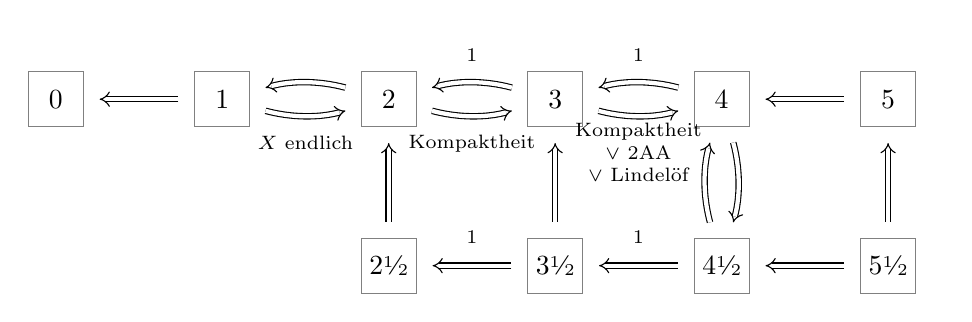
\begin{tikzpicture} [
			axiom/.style={rectangle,draw=black!50},
			node distance=14mm,
			minimum size=7mm,
			inner sep=1mm,
			implies/.style={double,-implies,double equal sign distance, shorten >=2mm, shorten <=2mm},
			label/.style={font=\scriptsize,auto,swap},
			bend angle=15,
		]
		\node[axiom] (T0) {\SepAxiom0};
		\node[axiom] (T1) [right=of T0] {\SepAxiom1};
		\node[axiom] (T2) [right=of T1] {\SepAxiom2};
		\node[axiom] (T3) [right=of T2] {\SepAxiom3};
		\node[axiom] (T4) [right=of T3] {\SepAxiom4};
		\node[axiom] (T5) [right=of T4] {\SepAxiom5};
		\node[axiom] (T2h) [below=of T2] {\SepAxiom{2\sfrac12}};
		\node[axiom] (T3h) [below=of T3] {\SepAxiom{3\sfrac12}};
		\node[axiom] (T4h) [below=of T4] {\SepAxiom{4\sfrac12}};
		\node[axiom] (T5h) [below=of T5] {\SepAxiom{5\sfrac12}};
		\draw[implies] (T1) to node[label] {} (T0);
		\draw[implies] (T2) to[bend right] node[label] {} (T1);
		\draw[implies] (T1) to[bend right] node[label] {$X$ endlich} (T2);
		\draw[implies] (T3) to[bend right] node[label] {\SepAxiom1} (T2);
		\draw[implies] (T2) to[bend right] node[label] {Kompaktheit} (T3);
		\draw[implies] (T4) to[bend right] node[label] {\SepAxiom1} (T3);
		\draw[implies] (T3) to[bend right] node[label,align=center] {Kompaktheit \\ $\lor$ 2AA \\ $\lor$ Lindelöf} (T4);
		\draw[implies] (T5) to node[label] {} (T4);
		\draw[implies] (T3h) to node[label] {\SepAxiom1} (T2h);
		\draw[implies] (T4h) to node[label] {\SepAxiom1} (T3h);
		\draw[implies] (T5h) to node[label] {} (T4h);
		\draw[implies] (T2h) to node[label] {} (T2);
		\draw[implies] (T3h) to node[label] {} (T3);
		\draw[implies] (T4h) to[bend left] node[label] {} (T4);
		\draw[implies] (T4) to[bend left] node[label] {} (T4h);
		\draw[implies] (T5h) to node[label] {} (T5);
	\end{tikzpicture}
	\caption{Zusammenhänge zwischen Trennungseigenschaften}
	\label{fig:separation_axioms}
\end{figure}

\begin{df}
	Ein topologischer Raum $(X, \scr T)$ heißt
	\begin{enumerate}[1)]
		\item
			\emph{hausdorffsch}, wenn $\SepAxiom2$ erfüllt ist,
		\item
			\emph{regulär}, wenn \SepAxiom1 und \SepAxiom3 erfüllt sind,
		\item
			\emph{vollständig regulär}, wenn \SepAxiom1 und \SepAxiom{3\sfrac 12} erfüllt sind,
		\item
			\emph{normal}, wenn \SepAxiom1 und \SepAxiom4 erfüllt sind,
		\item
			\emph{vollständig normal}, wenn \SepAxiom1 und \SepAxiom5 erfüllt sind,
		\item
			\emph{perfekt normal}, wenn \SepAxiom1 und \SepAxiom{5\sfrac 12} erfüllt sind.
	\end{enumerate}
\end{df}

\begin{lem}[Tychonoff]
	2AA und \SepAxiom3 impliziert \SepAxiom4.
\end{lem}

\begin{st}[Urysohn]
	Sei $(X, \scr T)$ ein \SepAxiom4-Raum.
	Dann gilt \SepAxiom{4\sfrac 12}.
	\begin{note}
		\SepAxiom4 besagt insbesondere:
		Zu $A \subset O$ mit $A$ abgeschlossen und $O$ offen existiert $U$ offen mit $A \subset U \subset  \_{U} \subset O$.
	\end{note}
	\begin{proof}
		Sei $A, B \subset X$ abgeschlossen, $A \cap B = \emptyset$.
		Setze $\_{A_0} = A_0 := B$, $A_1 := X \setminus A$.
		$A_1$ ist offene Umgebung von $\_{A_0}$.
		Sei $f_0: X \to [0,1]$ definiert durch $f_0|_{A_1} = 0, f_0|_{A} = 1$.
		Nach \SepAxiom4 existiert $A_{\f 12} \in \scr T$ mit
		\[
			B = \_{A_0} \subset A_{\f 12} \subset \_{A_{\f 12}} \subset A_1
		\]
		Sei $f: X \to [0,1], f|_{A_{\f 12}} = 0, f|_{A_1 \setminus A_{\f 12}} = \f 12, f|_A = 1$.

		Per Induktion erhalten wir $A_{\f {k}{2^n}} \in \scr T$ mit
		\[
			B = \_{A_{\f 0{2^n}}} \subset A_{\f 1{2^n}} \subset \_{A_{\f 1{2^n}}}
			\subset \dotsb \subset
			\_{A_{\f{2^n - 1}{2^n}}}
			\subset A_{\f {2^n}{2^n}}
			= X \setminus A.
		\]
		Wir definieren $f_n : X \to [0,1]$ durch $f|_{A_{\f 1{2^n}}} = 0$,
		\[
			f\Big|_{A_{\f {k+1}{2^n}} \setminus A_{\f {k}{2^n}}}
			= \f k{2^n}
		\]
		und $f|_A = 1$.
		Für jedes $x \in X$ ist $f_n(x) \in [0,1]$ monoton wachsend in $n$.
		Also $f_n(x) \to f(x) \in [0,1]$, $f_n$ konvergiert gleichmäßig gegen $f: X \to [0,1]$.

		Für $n \in \N$ wird $X$ überdeckt durch
		\begin{align*}
			U_n^0 &= A_{\f 1{2^n}} \\
			U_n^1 &= A_{\f 2{2^n}} \setminus A_{\f 0{2^n}} \\
			\vdots \quad &= \qquad \vdots \\
			U_n^{2^n-1} &= A_{\f {2^n}{2^n}} \setminus A_{\f {2^n-2}{2^n}} \\
			U_n^{2^n} &= X \setminus \_{A_{\f {2^n-1}{2^n}}}.
		\end{align*}
		Auf $U_n^k$ schwankt $f_n$ um höchstens $2^{-n}$ und $f$ um höchstens $2\cdot 2^{-n}$.
		Zu jedem $x \in X$ und $\eps > 0$ wählen wir $n \in \N$ so dass $2^{-n+1} < \eps$.
		Es gilt $x \in U_n^k$ für ein $k$.
		Dann ist
		\[
			f(U_n^k) \subset ]f(x) - \eps, f(x) + \eps[.
		\]
		Das bedeutet, $f$ ist stetig.
		% fixme: prüfen
	\end{proof}
\end{st}

\begin{lem}
	Sei $A \subset X$ abgeschlossen und $\phi: A \to [-s, s]$ stetig.
	Dann existiert $\Phi: X \to [-s, s]$ stetig mit
	\[
		|\phi(a) - \Phi(a)| \le \f 23 s
	\]
	für alle $a \in A$.
	\begin{proof}
		Setze $M := \phi^{-1}([-s, - \f s3]), N := \phi^{-1}([\f s3, s])$.
		$M, N$ sind ebgeschlossen.
		Nach Urysohn existiert $\Phi: X \to [-\f s3, \f s3]$ mit $\Phi|_M = - \f s3, \Phi|_N = \f s3$.
	\end{proof}
\end{lem}

\begin{st}[Tietze]
	Sei $(X, \scr T)$ ein \SepAxiom4-Raum.
	Ist $A \subset X$ abgeschlossen und $f: A \to [a,b]$ stetig.
	Dann existiert $F: X \to [a,b]$ stetig mit $F|_A = f$.
	\begin{proof}
		Sei \oBdA $[a,b] = [-1,1]$.
		Zu $f: A \to [-1,1]$ existiert $\Phi_0 : X \to [-\f 13, \f 13]$ wie im Lemma.
		Der Fehler auf $A$ ist $\phi_0 = f - \Phi_0|_A : A \to [-\f 23, \f 23]$.
		Zu $\phi_0$ existiert $\Phi_1: X \to [-\f 13 \cdot \f 23, \f 13 \cdot \f 23]$ wie im Lemma. % fixme: ref

		Per Induktion für $n \in \N$ ergibt sich der verbleibende Fehler als
		\[
			\phi_n = f - \Big( \Phi_0 + \Phi_1 + \dotsb + \Phi_n \Big)\Big|_A
			: A \to [-(\f 23)^{n+1}, (\f 23)^{n+1}.
		\]
		Dank Lemma existiert $\Phi_{n+1}: X \to [-\f 13(\f 23)^{n+1}, \f 13 (\f 23)^{n+1}]$.
		Damit konvergiert $F_n = \sum_{k=0}^n \Phi_n$ gleichmäßig auf $X$, denn
		\[
			\sum_{k=0}^n \|\Phi_k\|
			\le \sum_{k=0}^\infty \f 13 (\f 23)^k
			= 1.
		\]
		Die Grenzfunktion $F: X \to \R$ ist also stetig als glechimäßiger Grenzwert stetiger Funktionen und erfüllt
		\[
			\|F\| \le \sum_{k=0}^\infty \|\Phi_k\| = 1,
		\]
		also $F(X) \subset [-1, 1]$.
		Wegen $\phi_n \to 0$ gilt $f - F_n|_A \to 0$, also $F|_A = f$.
	\end{proof}
\end{st}

\begin{kor}
	Sei $(X, \scr T)$ ein \SepAxiom4-Raum.
	Ist $A \subset X$ abgeschlossen, $f: A \to \R^n$ stetig, so existiert $F: X \to \R^n$ stetig mit $F|_A = f$.
	\begin{note}
		Der Zielraum $\R^n$ ist wesentlich.
		Sei $Y = \R \setminus \{0\}, X = [-1,1], A = \{-1, 1\}, f: A \to Y, f(\pm 1) := \pm 1$.
		Hier existiert nach Zwischenwertsatz keine stetige Fortsetzung.
	\end{note}
\end{kor}

\begin{st}[Metrisierbarkeitssatz von Urysohn, 1924]
	Sei $(X, \scr T)$ ein topologischer Raum, der dem zweiten Abzählbarkeitsaxiom genügt.
	Dann sind äquivalent
	\begin{enumerate}[1)]
		\item
			$X$ ist metrisierbar,
		\item
			$X$ ist regulär, d.h. \SepAxiom1 und \SepAxiom3 ist erfüllt,
		\item
			$X$ ist normal, d.h. \SepAxiom1 und \SepAxiom4 ist erfüllt,
		\item
			$X$ ist homöomorph zu einem Teilraum von $[0,1]^\N$ (Hilbertwürfel).
	\end{enumerate}
	\begin{proof}
		\begin{segnb}[„(1)$\implies$(2)“]
			klar
		\end{segnb}
		\begin{segnb}[„(2)$\implies$(3)“]
			Folgt mit Lemma von Tychonoff. % fixme: ref
		\end{segnb}
		\begin{segnb}[„(3)$\implies$(4)“]
			Sei $\scr B$ eine abzählbare Basis.
			Sei $I$ die abzählbare Menge aller Paare $i = (U,V)$ mit $U,V \in \scr B$ und $\_U \subset V$.

			Dank Urysohn existiert $f_i: X \to [0,1]$ mit $f_i|_{\_U} = 0, f_i|_{X \setminus V} = 1$.
			Wir erhalten hieraus $h: X \to [0,1]^I, h(x) = (f_i(x))_{i \in I}$.
			Dies ist eine Einbettung.
		\end{segnb}
		\begin{segnb}[„(4)$\implies$(1)“]
			$[0,1]^\N$ ist metrisierbar, etwa durch
			\[
				d(x,y) = \sum_{k=0}^\infty 2^{-k-1} |x_i - y_i|,
			\]
			siehe Übungsaufgabe. % fixme: ref
		\end{segnb}
	\end{proof}
\end{st}

\chapter{Zusammenhang und Homotopie}

\coursetimestamp{26}{11}{2013}

\section{Zusammenhang}

\begin{st}
	Für jeden topologischen Raum $(X, \scr T)$ sind folgende Aussagen äquivalent:
	\begin{enumerate}[(1)]
		\item
			Jede stetige Funktion $f: X \to \R$ hat die Zwischenwerteigenschaft
		\item
			Für $f: X \to \R$ stetig ist $f(X) \subset \R$ ein Intervall.
		\item
			Jede stetige Funktion $f: X \to \{0,1\}$ (diskret) ist konstant.
		\item
			Jede stetige Funktion $f: X \to Y$ in einen diskreten Raum $Y$ ist konstant.
		\item
			Für jede offene Zerlegung $X = A \dunion B$ gilt $A = \emptyset$ oder $B = \emptyset$.
	\end{enumerate}
	$(X, \scr T)$ mit diesen Eigenschaften nennen wir \emph{zusammenhängend}.
	\begin{proof}
		Wie im metrischen Fall.
	\end{proof}
\end{st}

\begin{ex}
	\begin{itemize}
			%fixme: diskret, indiskret
		\item
			Jedes Intervall $I \subset \R$ ist zusammenhängend (ZWS).
		\item
			$\R \setminus \{a\}$ ist nicht zusammenhängen, denn $\R \setminus \{a\} = \R_{<a} \dunion \R_{>a}$.
		\item
			$\Q$ ist unzusammenhängend.
	\end{itemize}
\end{ex}

\begin{st}
	Sei $(X, <)$ linear geordnet.
	Jedes Intervall $I \subset X$ ist zusammenhängend genau dann, wenn $X$ vollständig geordnet und dicht ist.
	\begin{proof}
		Wie in $\R$, bzw. $\Q$.
	\end{proof}
\end{st}

\begin{proof}
	\begin{itemize}
		\item
			$(\R, <)$ ist vollständig geordnet, also $I \subset \R$ zusammenhängend.
		\item
			$(\Q, <)$ ist nicht vollständig geordnet.
			Das Intervall $[0,1]_\Q$ ist nicht zusammenhängend, denn für $\xi \in [0,1] \setminus [0,1]_\Q$ ist
			\[
				[0,1]_\Q =
				\Set{ x \in \Q | 0 \le x < \xi }
				\dunion
				\Set{ x \in \Q | \xi < x \le 1 }
			\]
			eine offene Zerlegung.
	\end{itemize}
\end{proof}

\begin{st}
	Ist $f: X \to Y$ stetig und $X$ zusammenhängend, so auch $f(X)$.
	\begin{proof}
		Ist $f(X) = A \dunion B$ offene Zerlegung, so auch $X = f^{-1}(A) \dunion f^{-1}(B)$, also $A = \emptyset$ oder $B = \emptyset$.
	\end{proof}
\end{st}

\begin{lem}
	Sei $X$ ein topologischer Raum und $A_i \subset X$ für $i \in I$ zusammenhängend.
	Für jedes Paar $i,j \in I$ existiere eine Kette $i = i_0 , i_1, \dotsc, i_n = j$ in $I$ mit $A_{i_{k-1}} \cap A_{i_k} \neq \emptyset$ für $k = 1, \dotsc, n$.

	Dann ist $A = \bigcup_{i\in I} A_i$ zusammenhängend.
	\begin{proof}
		Sei $f: A \to \{0,1\}$ stetig.
		Dann ist $f_i := f|_{A_i}: A_i \to \{0,1\}$ stetig, also $f_i$ konstant, kurz $f_i = c_i$.
		Für $i = i_0, \dotsc, i_n = j$ wie oben gilt dann $c_i = \dotsb = c_j$.
	\end{proof}
\end{lem}

\begin{lem}
	Seien $X_1, \dotsc, X_n$ zusammenhängend, so auch $X = X_1 \times \dotsb \times X_n$.
	\begin{proof}
		Sei $a \in X$ und $f: X \to \{0,1\}$ stetig.
		Zu $b \in X$ betrachte
		\begin{align*}
			A_i &= \{ b_1 \} \times \dotsb \times \{b_{i-1}\} \times X_i \times \{a_{i+1}\} \times \dotsb \times \{a_n\} \\
			&\homeomorphic X_i.
		\end{align*}
		Es gilt $a \in A_1$, $b \in A_n$ und $A_{i-1} \cap A_i \ni (b_1, \dotsc, b_{i-1}, a_i, \dotsc, a_n)$.
		Nach dem Lemma ist $A_1 \cup \dotsb \cup A_n$ zusammenhängend, also $f(b) = f(a) = \const$.
	\end{proof}
\end{lem}

\begin{lem}
	Sei $(X, \scr T)$ ein topologischer Raum, $A \subset X$ zusammenhängend und $A \subset B \subset \_A$.
	Dann ist auch $B$ zusammenhängend.
	\begin{proof}
		Sei $f: B \to \{0,1\}$ stetig, dann ist $f|_A = c$ konstant.
		Die Abbildungen $f, c: B \to \{0,1\}$ sind stetig und stimmen auf $A$ überein.
		$A$ ist dicht in $B$ und $\{0,1\}$ ist hausdorffsch.
		Also gilt $f=c$.
	\end{proof}
\end{lem}

\begin{st}
	Sei $(X_i)_{i\in I}$ eine Familie topologischer Räume mit $X_i \neq \emptyset$.
	Der Produktraum $X = \prod_{i\in I} X_i$ ist genau dann zusammenhängend, wenn jedes $X_i$ zusammenhängend ist.
	\begin{proof}
		\begin{segnb}[„$\implies$“]
			Klar, da $p_i: X \to X_i$ stetig und surjektiv ist.
		\end{segnb}
		\begin{segnb}[„$\implies$“]
			Sei $a \in X$.
			Für $J \subset I$ endlich sei
			\begin{align*}
				A_J &:= \prod_{i\in I} A_i, &
				A_j &:= \begin{cases}
					X_j & j \in J \\
					\{a_j\} & j \in I \setminus J
				\end{cases}.
			\end{align*}
			$A_j$ ist zusammenhängend nach obigem Lemma.
			Damit ist auch $A = \bigcup_{J} A_J$ zusammenhängend, denn $A_J \cap A_j \ni \{a\}$.

			Es gilt außerdem $\_A = X$:
			Jede offen Menge $U \subset X$ enthält $\prod_{i \in I} U_i$, wobei $U_i \subset X_i$ offen und $U_i = X_i$ für $i \in I \setminus J$ außerhalm einer endlichen Menge.
			Ist $U$ nicht-leer, dann gilt $U_i \neq \emptyset$ für alle $i \in I$.
			Demnach existiert $b \in U$ mit $b_j \in U_j$ für alle $j \in J$ und $b_i = a_i$ für alle $i \in I \setminus j$.
			Damit gilt $b \in A_J$, also $b \in U \cap A$.
		\end{segnb}
	\end{proof}
\end{st}

%fixme \eqq ===
\begin{df}
	Sei $(X, \scr T)$ ein topologischer Raum.
	Für $x,y \in X$ definieren wir $x \eqq y$ durch die Bedingung, dass $x,y$ in einer zusammenhängend Teilmenge von $X$ liegen.
	Dies ist eine Äquivalenzrelation.
	Die Äquivalenzklasse $\scr Z(x)$ von $x$ heißt \emph{(Zusammenhangs)komponente} von $x$ in $X$.
	Die definiert die Zerlegung
	\[
		\scr Z(X) := \{ \scr Z(x) : x \in X \}.
	\]
\end{df}

\begin{ex}
	\begin{itemize}
		\item
			$X$ ist zusammenhängend genau dann, wenn $\scr Z(X) = \{X\}$.
		\item
			$\scr Z(\R \setminus \{0\}) = \{ \R_{<0}, \R_{>0} \}$.
		\item
			$\scr Z(\Q) = \{ \{x\} : x \in \Q \}$.
	\end{itemize}
\end{ex}

\begin{st}
	\begin{enumerate}[(1)]
		\item
			$\scr Z(x)$ ist der größte zusammenhängende Teilraum von $X$, der $x$ enthält.
		\item
			Jede Komponente $\scr Z(x)$ ist abgeschlossen.
		\item
			Ist die Zerlegung $\scr Z(X)$ endlich, so ist jede Komponente offen und $X = \bigdunion \scr Z(X)$ ist eine Summentopologie.
	\end{enumerate}
\end{st}

\begin{st}
	\begin{enumerate}[(1)]
		\item
			Ist $f: X \to Y$ stetig, so gilt $f(\scr Z(x)) \subset \scr Z(f(x))$.
		\item
			Wir erhalten hieraus $\scr Z(f): \scr Z(X) \to \scr Z(Y): \scr Z(x) \mapsto \scr Z(f(x))$.
		\item
			Es gilt $\scr Z(\Id_X) = \Id_{\scr Z(X)}$ und $\scr Z(g\circ f) = \scr Z(g) \circ \scr Z(f)$.
	\end{enumerate}
	\begin{proof}
		(1) und (2) sind klar nach den vorigen Ergebnissen, zeige noch (3).
		Es gilt
		\begin{align*}
			\scr Z(g\circ f) (\scr Z(x))
			&= \scr Z(g(f(\scr Z(x)))) \\
			&= \scr Z(g) (\scr Z(f(\scr Z(x)))) \\
			&= \scr Z(g)(\scr Z(f)(\scr Z(x))) \\
			&= (\scr Z(g) \circ \scr Z(f)) (\scr Z(x)).
		\end{align*}
	\end{proof}
\end{st}


\section{Wegzusammenhang}

Analog zum Weg in metrischen Räumen definieren wir im Wege in topologischen Räumen.

\begin{df}
	Ein \emph{Weg} im topologischen Raum $(X, \scr T)$ ist eine stetige Abbildung $\gamma: [0,1] \to X$.
	Dabei heißt $\gamma(0) = a$ \emph{Anfangspunkt} und $\gamma(1) = b$ \emph{Endpunkt}.

	Der Raum $X$ heißt \emph{wegzusammenhängend}, wenn zu jedem Paar $a,b \in X$ ein Weg von $a$ nach $b$ in $X$ existiert (d.h. $\gamma:[0,1] \to X$ stetig mit $\gamma(0) = a, \gamma(1) = b$).

	Wir definieren die Menge aller Wege $P(X)$ und die Menge aller Wege von $a$ nach $b$, $P(X, a, b)$ als
	\begin{align*}
		P(X) &= \scr C ([0,1], X), \\
		P(X, a, b) &= \{ \gamma : [0,1] \to X \text{ stetig } : \gamma(0) = a, \gamma(1) = b \}.
	\end{align*}
	Außerdem folgende Abbildungen, bzw. Operatoren:
	\begin{enumerate}[1)]
		\item
			$X \injto P(X), a \mapsto \const_{[0,1]}^a$,
		\item
			$\_\  : P(X, a, b) \to P(X, b, a), \_\gamma(t) := \gamma(1-t)$,
		\item
			$\ast: P(X, a, b) \times P(X, b, c) \to P(X, a, c)$ durch
			\[
				(\gamma_1 \ast \gamma_2)(t) := \begin{cases}
					\gamma_1 (2t) & 0 \le t \le \f 12 \\
					\gamma_2 (2t - 1) & \f 12 \le t \le 1
				\end{cases}.
			\]
	\end{enumerate}
\end{df}

\begin{df}
	Wir nennen $x,y \in X$ \emph{verbindbar} in $X$ (durch einen Weg in $X$), wenn ein Weg $\gamma: [0,1] \to X$ von $\gamma(0) = x$ nach $\gamma(1) = y$ existiert.
	Dies ist eine Äquivalenzrelation.

	Die Äquivalenzklasse $[x]$ von $x$ heißt \emph{Weg(-Zusammenhangs)komponente}.
	Dies definiert die Zerlegung
	\[
		\pi_0 (X) := \{ [x] : x \in X \}.
	\]
	$X$ heißt \emph{wegzusammenhängend}, wenn $\pi_0(X) = \{X\}$.
\end{df}

\begin{ex}
	\begin{itemize}
		\item
			Jedes Intervall $I \subset \R$ ist wegzusammenhängend.
		\item
			Jede sternförmige Menge $X \subset \R^n$ ist wegzusammenhängend.
		\item
			$\S^n \subset \R^{n+1}$ ist wegzusammenhängend für $n \ge 1$.
	\end{itemize}
\end{ex}

\begin{st}
	Wegzusammenhang impliziert Zusammenhang, aber nicht umgekehrt.
	\begin{proof}
		Wie im metrischen Fall.
		Gegenbeispiel folgt. % fixme: ref
	\end{proof}
\end{st}

\begin{ex}
	Sei
	\begin{align*}
		A &:= \Set{ (x, \sin( \f {\pi}x)) | x \in ]0,1] } \\
		B &:= \{0\} \times [-1, 1]
	\end{align*}
	$C = \_A = A \cup B$ ist zusammenhängend, aber nicht wegzusammenhängend.
\end{ex}

\coursetimestamp{02}{12}{2013}

\begin{st}
	Ist $f: X \to Y$ stetig und $X$ wegzusammenhängend, so auch $f(X)$.
\end{st}

\begin{st}
	Seien $(X_i, \scr T_i)$ mit $X_i \neq \emptyset$ topologische Räume.
	Genau dann ist $\prod_{i \in I} X_i$ wegzusammenhängend, wenn jeder Raum $X_i$ dies ist.
	\begin{st}
		Folgt mit universeller Abbildungseigenschaft und dem letzten Satz.
	\end{st}
\end{st}

\begin{st}
	\begin{enumerate}[1)]
		\item
			Ist $f: X \to Y$ stetig, so gilt
			\[
				f([a]_X) \subset [f(a)]_Y.
			\]
		\item
			Wer erhalten mit 1) die Abbildung $\pi_0(f): \pi_0(X) \to \pi_0(Y): [a]_X \mapsto [f(a)]_Y$.
		\item
			Es gilt $\pi_0(\Id_X) = \Id_{\pi_0(X)}$ und $\pi_0(g \circ f) = \pi_0(g) \circ \pi_0(f)$.
			Das folgende Diagramm kommutiert:
			\[
				\begin{tikzcd}[row sep=small]
					X \arrow{dr}{f} \arrow{dd}[left]{g\circ f} \arrow{rr} &  & \pi_0(X) \arrow{dr}{\pi_0(f)} & \\
					& Y \arrow{dl}{g} \arrow{rr} &  & \pi_0(Y) \arrow{dl}{\pi_0(g)}\\
					Z \arrow{rr}  & & \pi_0(Z) \arrow[leftarrow, crossing over]{uu}[yshift=5mm]{\pi_0(g\circ f)} &
				\end{tikzcd}.
			\]
	\end{enumerate}
	\begin{proof}
		\begin{enumerate}[1),start=3]
			\item
				Es gilt
				\begin{align*}
					\pi_0(g\circ f)([a]_X)
					&= [(g\circ f)(a)]_Z
					= [g(f(a))]_Z
					= \pi_0(g)([f(a)]_Y) \\
					&= \pi_0(g)(\pi_0(f)([a]_X))
					= (\pi_0(g)\circ \pi_0(f))([a]_X).
				\end{align*}
		\end{enumerate}
	\end{proof}
\end{st}


\section{Lokaler Zusammenhang}


\begin{df}
	Ein topologischer Raum $(X, \scr T)$ heißt \emph{lokal (weg-)zusammenhängend} in $a \in X$, wenn jede offene Umgebung von $a$ in $X$ eine (weg-)zusammenhängende offene Umgebung enthält.
\end{df}

\begin{ex}
	\begin{itemize}
		\item
			$\R^n$ ist lokal wegzusammenhängend, denn $B(a,\eps)$ ist sternförmig und somit wegzusammenhängend.
			Ebenso jeder topologische Vektorraum (ausgeglichene Umgebung ist sternförmig).
		\item
			Ist $X$ lokal wegzusammenhängend, so auch jede offene Teilmenge $U \subset X$.
	\end{itemize}
\end{ex}

\begin{ex}
	\begin{itemize}
		\item
			Die „Sinuskurve des Topologen“ % fixme: ref
			ist zusammenhängend, aber nicht lokal zusammenhängend.
		\item
			Der „rationale Kamm“
			\[
				X = ([0,1] \times \{0\}) \cup ([0,1]_\Q \times [0,1])
			\]
			ist wegzusammenhängend, aber nicht lokal wegzusammenhängend.
		\item
			$X = [0,1] \cup [2,3]$ ist lokal (weg-)zusammenhängend, aber nicht global (weg-)zusammenhängend.
	\end{itemize}
\end{ex}

Zu jedem Raum $X$ haben wir die Zerlegungen $X = \bigdunion \scr Z(X)$ und $X = \bigdunion \pi_0(X)$.

\begin{st}
	Ist $X$ lokal zusammenhängend, so ist die Zerlegung $X = \bigdunion \scr Z(X)$ offen.

	Ist $X$ lokal wegzusammenhängend, so ist die Zerlegung $X = \bigdunion \pi_0(X)$ offen.
	In diesem Fall gilt $\pi_0(X) = \scr Z(X)$.
	\begin{proof}
		Leicht nachzuvollziehen.
	\end{proof}
\end{st}


\section{Homotopie stetiger Abbildungen}


\begin{df}
	Eine \emph{Homotopie} ist eine stetige Abbildung $H: [0,1] \times X \to Y$.
	Für jedes $t \in [0,1]$ ist dann $H_t: X \to Y$ mit $H_t(x) := H(t,x)$ stetig.

	Zwei stetige Abbildungen $f,g : X \to Y$ heißen \emph{homotop} in $Y$, wenn es eine Homotopie $H: [0,1] \times X \to Y$ mit $H_0 = f$ und $H_1 = g$ gibt.
	Wir schreiben dann $H: f \homotopic g$, oder $f\homotopic g$

	Ist $f: X \to  Y$ homotop zu $\const_X^{\{\ast\}}: X \to \{\ast\} \subset Y$, so nennen wir $f$ \emph{nullhomotop}, Kurz $f \homotopic \ast$.
	Der Raum $X$ heißt \emph{zusammenziehbar}, wenn $\Id_X \homotopic \ast$.
\end{df}

\begin{ex}
	Sei $X \subset \R^n$ sternförmig bezüglich $a \in X$ (z.B. $X = \R^n, a = 0$).

	Dann ist $X$ zusammenziehbar mittels $H: [0,1] \times X \to X, H(t,x) = (1-t)x + ta$.

	Es gilt $H_0 = \Id_X, H_1 = \const_X^{a}$.
	$H$ ist wohldefiniert und stetig für alle $(t,x) \in [0,1] \times X$.
\end{ex}

\begin{st}
	Seien $f,g : X \to \S^n$ stetig und nirgends antipodal, d.h. $f(x) \neq -g(x)$ für alle $x \in X$.
	Dann sind $f$ und $g$ homotop in $\S^n$ mittels
	\[
		H(t,x) := \f {(1-t)f(x) - tg(x)}{|(1-t)f(x) - tg(x)|}.
	\]
	\begin{proof}
		klar
	\end{proof}
\end{st}

\begin{kor}
	Ist $f: X \to \S^n$ stetig, aber nicht surjektiv, so gilt $f \homotopic *$.
	\begin{proof}
		Es gibt zwei Möglichkeiten, dies zu beweisen:
		\begin{enumerate}[1.]
			\item
				Wähle $a \in \S^n \setminus (X)$ und $g = \const_X^{-a}$, dann ist $f \homotopic g$ wie im letzten Satz.
			\item
				Mittels stereographischer Projektion.
				Für $a \in \S^n \setminus f(X)$ ist $\S^n \setminus \{a\} \homeomorphic \R^n \homotopic *$ wie im Beispiel.
		\end{enumerate}
	\end{proof}
\end{kor}

\begin{df}
	\begin{enumerate}[(1)]
		\item
			Zu $f: X \to Y$ haben wir $H: f \homotopic f$ mit $H(t,x) = f(x)$.
		\item
			Zu $H: f \homotopic g$ definieren wir $\_H: g \homotopic f$ mit $H(t,x) := H(1-t,x)$.
		\item
			Zu $H: f \homotopic g$ und $K: g\homotopic h$ definieren wir $(H \ast K) : f \homotopic h$ durch
			\[
				(H \ast K)(t,x) = \begin{cases}
					H(2t, x) & 0 \le t \le \f 12 \\
					K(2t-1), x) & \f 12 \le t \le 1
				\end{cases}.
			\]
	\end{enumerate}
	Homotopie ist eine Äquivalenzrelation.
\end{df}

\begin{df}
	Die Menge der Homotopieklassen von $\scr C(X, Y)$ bezeichnen wir mit
	\[
		[X,Y] := \scr C(X, Y) / \homotopic.
	\]
\end{df}

%fixme : anmerkung zur notation
\begin{st}
	Aus $H: f_0 \homotopic f_1 : X \to Y$ und $K: g_0 \homotopic g_1: Y \to Z$ folgt $L: g_0 \circ f_0 \homotopic g_1 \circ f_1$ mittels
	\[
		L(t, x) = K(t, H(t,x)).
	\]
	Wir schreiben auch $L_t = K_t \circ H_t$.
\end{st}

\begin{kor}
	Wir haben eine Kategorie \emph{Toph}:
	\begin{itemize}
		\item
			Objekte sind topologische Räume $X, Y, Z, \dotsc $,
		\item
			Morphismen sind Homotopieklassen $[f]$ von stetigen Abbildungen $f: X \to Y$,
		\item
			Die Komposition ist $[g] \circ [f] = [g\circ f]$.
	\end{itemize}
\end{kor}

\begin{st}
	Der Funktor $\pi_0: \mathrm{Top} \to \mathrm{Set}$ ist homotopie-invariant, d.h. aus $f \homotopic g$ folgt $\pi_0(f) = \pi_0(g)$.
	\[
		\begin{tikzcd}[row sep=tiny]
			\mathrm{Top} \arrow{dr}{\pi_0} \arrow{dd}[left]{q} & \\
			& \mathrm{Set} \\
			\mathrm{Toph} \arrow{ur}[below]{\pi_0} & \\
		\end{tikzcd}.
	\]
\end{st}

\begin{df}
	Zwei Räume $X, Y$ heißen \emph{homotopie-äquivalent}, geschrieben $X \homotopic Y$, wenn es stetige Abbildungen $f: X \to Y$ und $g: Y \to X$ gibt mit $g \circ f \homotopic \Id_X$ und $f \circ g \homotopic \Id_Y$.
\end{df}

\begin{ex}
	\begin{enumerate}[1)]
		\item
			Falls $X \homeomorphic Y$, dann auch $X \homotopic Y$.
		\item
			Aus $X \homotopic Y$ folgt nicht $X \homeomorphic Y$, z.b. $\R \not \homeomorphic \R^2$, aber $\R \homotopic \R^2 \homotopic \ast$.
	\end{enumerate}
\end{ex}

\begin{ex}
	$X = \S^n$ und $Y = \R^{n+1} \setminus \{0\}$ sind homotopie-äquivalent.
	\begin{proof}
		Sei $f: X \injto Y$ die Inklusion und $g: Y \to X, g(y) = \f y{|y|}$.
		Es gilt $g \circ f = \Id_X$ ($g$ ist \emph{Retrakt}) und $f \circ g \homotopic \Id_Y$ mittels
		\[
			H(t,y) = ty + (1-t) g(y) \in Y.
		\]
		$H$ ist \emph{(starker) Deformationsretrakt}.
	\end{proof}
\end{ex}





\end{document}
